\documentclass[11pt,a4paper]{article}
\usepackage[margin=1in]{geometry}
\usepackage{graphicx}
\usepackage{booktabs}
\usepackage{amsmath}
\usepackage{float}
\usepackage{hyperref}
\usepackage{caption}
\usepackage{subcaption}

\title{Reproduction Report: Optimization-Driven Quantum Circuit Reduction\\[4pt]
\large (with an exact engine that improves on the paper's ion-trap results)}
\author{Arnav Kapoor 23060}
\date{\today}

\begin{document}
\maketitle

\begin{abstract}
This report documents a complete, reproducible implementation of
\emph{Optimization driven quantum circuit reduction} (Rosenhahn, Osborne and
Hirche, New J.\ Phys.\ 27 (2025) 104509), from the paper's MATLAB demo through a
Python reimplementation, benchmark infrastructure, figure generation, and
baseline/future-work artifacts. Beyond reproduction, it adds an \textbf{original
exact engine} built on a bit-exact symplectic (Clifford) lookup. On the paper's
ion-trap benchmark (4 qubits, 300-gate random circuits, Table 6) this engine
reduces further than the paper's reported ``Ours'': a mean of \textbf{73.0
gates} (with 27.4 RXX) versus the paper's \textbf{111 gates} (43 RXX), while
remaining bit-exact (no 1e-5 tolerance anywhere). On the NISQ gate set a gap
remains (159 vs.\ 107); \S\ref{sec:comparison} analyses both results honestly,
including a baseline-fidelity check against the paper's own qiskit baselines.
On the paper's 5-qubit demo circuit the numeric port reaches 228 gates under
strict (1e-5) verification, matching the paper-style protocol.
\end{abstract}

\section{Motivation and objective}
The paper's core idea is to reduce a transpiled circuit by \emph{local
replacement}: sample a contiguous block of gates, look it up in a precomputed
compute graph of equivalent (shorter) circuits, and substitute if the unitary
action is preserved up to global phase. My goal was to (i) reproduce that
protocol faithfully, (ii) go one step further and implement an exact,
non-tolerance-based engine, and (iii) run the paper's own benchmark protocol
(Tables 6/7) head-to-head against the paper's reported numbers on identical
inputs.

The repository is organised for a clean GitHub handoff:
\begin{itemize}
    \item \texttt{paper\_demo/QCOptimDemo/} --- reference MATLAB demo from the paper,
    \item \texttt{src/qcr\_repro/} --- Python package (token model, numeric
      compute-graph database, exact symplectic engine, reducers, QASM I/O),
    \item \texttt{scripts/} --- benchmarks, figure generation, report builders,
    \item \texttt{results/} --- benchmark outputs organised by protocol
      (\texttt{paper\_protocol\_1e-5}, \texttt{paper\_protocol\_1e-3},
      \texttt{baselines}, \texttt{costaware\_quick}, \texttt{comparison}),
    \item \texttt{figures/} --- all generated figures (1--6 reproduction, 7--9 comparison),
    \item \texttt{report/} --- this report and its data,
    \item \texttt{future\_work/} --- baseline parity and hardware-metrics probes.
\end{itemize}

\section{Workflow and implementation decisions}
\subsection{Stepwise execution log}
\begin{table}[H]
\centering
\caption{Reproduction workflow and rationale.}
\label{tab:workflow}
\begin{tabular}{p{0.13\linewidth}p{0.39\linewidth}p{0.41\linewidth}}
\toprule
Phase & What I did & Why I did it \\
\midrule
1 & Parsed the paper and extracted algorithmic requirements (V1/V2/V3 variants, gate sets, tolerances). & I needed a testable specification before writing any code. \\
2 & Set up a clean Python environment and project scaffold. & Reproducibility requires deterministic dependencies and scripted execution. \\
3 & Integrated the \texttt{QCOptimDemo} archive and inspected the MATLAB scripts. & The archive is the closest available ground-truth implementation reference. \\
4 & Ported the MATLAB demo logic to Python (QASM parsing, local remap, compute-graph lookup, replacement loop). & I wanted an executable, inspectable baseline in a modern workflow. \\
5 & Added equivalence checks and ran strict vs.\ loose tolerance validation. & Numeric tolerance strongly affects whether reductions are accepted. \\
6 & Built an \textbf{exact symplectic engine} (signed-tableau keyed lookups) and a cost-aware objective. & Removes tolerance fragility and targets the paper's deferred decoherence objective. \\
7 & Replicated the paper's Tables 6/7 protocol and compared head-to-head, including qiskit baselines. & Needed a direct verdict on identical inputs, with baseline-fidelity checks. \\
8 & Built figures/report and reorganised the repository for GitHub. & Evidence quality comparable to a lab handoff. \\
\bottomrule
\end{tabular}
\end{table}

\subsection{Technical implementation decisions}
The reduction pipeline follows the paper's local replacement concept:
\begin{enumerate}
    \item Parse the QASM circuit into gate tokens.
    \item Sample local contiguous blocks.
    \item Remap active wires to local coordinates (MATLAB \texttt{ExtractWireMap}/\texttt{WireMapF} analogue).
    \item Query a precomputed local compute-graph lookup.
    \item Accept a replacement only when it is shorter and unitary-consistent.
\end{enumerate}
Two decisions matter most. First, the \textbf{numeric engine} discretises
operators to the paper's angle sets ($\pm\pi/2$ for the ion-trap pool;
$\pm\pi/2, \pm\pi/4$ for NISQ) and verifies equivalence up to global phase at
1e-5. Second, the \textbf{exact engine} (\texttt{symplectic.py}) keys every
Clifford-pool lookup by a bit-exact signed tableau, so replacements are
equivalent \emph{by construction} and final verification is exact. We
additionally implement a \textbf{cost-aware objective}: every lookup minimises
(two-qubit count, length) --- the decoherence objective the paper lists as
future work --- including equal-length rewrites that cut RXX/CZ count, plus
structural passes (single-qubit clustering, 1-wire collapse, transport
shuffling, an RZ-across-CZ pass for NISQ, and equivalence-class escape moves
with restart-from-best).

\section{Reproduction results (paper protocol)}
\label{sec:protocol}
I benchmarked the numeric port over depths $\{3,4\}$, iteration budgets
$\{500,1000,1500\}$, and seeds $\{1,5,10\}$ (18 runs per tolerance setting) on
the paper's 5-qubit demo circuit (300 initial gates).
\begin{itemize}
    \item Best strict-valid run ($10^{-5}$): depth 4, iterations 1500, seed 10, end length \textbf{228}, runtime 29.8\,s.
    \item Best loose-valid run ($10^{-3}$): depth 4, iterations 1500, seed 5, end length \textbf{226}, runtime 2.4\,s.
\end{itemize}

\begin{table}[H]
\centering
\caption{Combined strict vs.\ loose tolerance results (3 seeds per configuration).}
\label{tab:combined}
\begin{tabular}{rrrrrrrrr}
\toprule
depth & iters & runs & best$_{strict}$ & mean$_{strict}$ & eq$_{strict}$ & best$_{loose}$ & mean$_{loose}$ & eq$_{loose}$ \\
\midrule
3 & 500  & 3 & 266 & 274.00 & 1.000 & 266 & 274.00 & 1.000 \\
3 & 1000 & 3 & 246 & 250.00 & 0.667 & 246 & 250.00 & 1.000 \\
3 & 1500 & 3 & 240 & 242.67 & 0.667 & 240 & 242.67 & 1.000 \\
4 & 500  & 3 & 262 & 265.33 & 1.000 & 262 & 265.33 & 1.000 \\
4 & 1000 & 3 & 238 & 243.33 & 1.000 & 238 & 243.33 & 1.000 \\
4 & 1500 & 3 & 226 & 231.33 & 0.667 & 226 & 231.33 & 1.000 \\
\bottomrule
\end{tabular}
\end{table}

Interpretation: the loose metric improves acceptance (1.000 pass rate vs.\
0.833) and is $\sim$13$\times$ faster, while strict verification is more
conservative and exposes fragile reductions --- a validation-fidelity tradeoff
that the paper's tolerance choice implicitly makes.

\section{Comparison with the paper}
\label{sec:comparison}
\subsection{Protocol}
\texttt{scripts/benchmark\_comparison.py} replicates the paper's Tables 6/7
protocol: 4 qubits, length-300 random circuits with the same per-gate-set input
composition (ion trap: uniform over RX/RY/RZ/RXX, reproducing the paper's
input row RX~78, RY~83, RZ~78, RXX~59; NISQ: CZ-weighted RX:1, RZ:1, CZ:2,
reproducing RX~108, RZ~109, CZ~82). Every circuit is reduced by our reducers
\emph{and} by the paper's baseline compilers (qiskit levels 1--3, optionally
BQSKit), then verified for unitary equivalence. The benchmark is crash-resistant
(multiprocessing falls back fork $\to$ spawn $\to$ sequential; database
construction happens on the parent so workers never pickle it).

\subsection{Ion trap (Table 6): our exact engine reduces further}
\begin{table}[H]
\centering
\caption{Mean total gates on identical circuits; ion-trap pool (RX/RY/RZ/RXX), 24 circuits, 15\,s budget each. Paper: Table 6 ``Ours'' (100 runs).}
\label{tab:ion}
\begin{tabular}{lrrrrr}
\toprule
method & RX & RY & RZ & RXX & total \\
\midrule
paper (``Ours'')   & 10  & 29  & 29  & 43 & 111 \\
exact\_len (ours)  & 4.5 & 20.3 & 22.0 & 32.7 & \textbf{79.5} \\
exact\_cost (ours) & 4.5 & 21.5 & 19.6 & \textbf{27.4} & \textbf{73.0} \\
qiskit L1 & 25.8 & 38.7 & 41.0 & 56.6 & 162.2 \\
qiskit L2 & 37.7 & 35.8 & 41.2 & 45.7 & 160.4 \\
qiskit L3 & 37.6 & 35.6 & 40.9 & 45.5 & 159.5 \\
\bottomrule
\end{tabular}
\end{table}

Our exact reducers improve on the paper's ``Ours'' in \emph{total} gates
($-31.5$ and $-38.0$) and in two-qubit gates (32.7 / 27.4 RXX vs.\ the paper's
43), with a 1.000 equivalence pass rate and best runs at 53 and 49 gates. The
cost-aware objective cuts a further $\sim$5 RXX at the same gate count --- the
decoherence-relevant direction the paper defers to future work.

One caveat must be stated honestly: our qiskit baselines (162.2 / 160.4 /
159.5) are \emph{lower} than the paper's reported qiskit baselines (196 / 204 /
204 on L1 / L2 / L3). Because our input composition matches the paper's (Table
6 input row), the likely explanations are compiler-version differences (our
qiskit 2.5 vs.\ the paper's toolchain) and/or residual protocol differences;
the improvement margin should be read with this in mind. The NISQ baseline
fidelity below is much tighter, which supports the comparison framework.

\subsection{NISQ (Table 7): gap remains}
\begin{table}[H]
\centering
\caption{Mean total gates; NISQ pool (RX/RZ/CZ), 12 circuits, 15\,s budget each. Paper: Table 7 ``Ours'' (100 runs).}
\label{tab:nisq}
\begin{tabular}{lrrrrr}
\toprule
method & RX & RZ & CZ & total \\
\midrule
paper (``Ours'')  & 45 & 19 & 43 & 107 \\
numeric\_len (ours)  & 65.8 & 42.2 & 50.3 & 158.4 \\
numeric\_cost (ours) & 66.9 & 42.6 & 50.2 & 159.8 \\
qiskit L1 & 60.5 & 68.8 & 71.4 & 200.7 \\
qiskit L2 & 61.2 & 41.8 & 50.4 & 153.3 \\
qiskit L3 & 61.2 & 41.8 & 50.4 & 153.3 \\
\bottomrule
\end{tabular}
\end{table}

On NISQ the paper's method is genuinely strong and we trail (159 vs.\ 107).
Two observations put this in context:
\begin{itemize}
    \item \textbf{Baseline fidelity is good.} Our qiskit L2/L3 means (153.3)
      closely match the paper's reported qiskit baselines (149), and L1 matches
      too (200.7 vs.\ 196) --- confirming the protocol reproduces the paper's
      input difficulty, so the NISQ head-to-head is fair.
    \item \textbf{The gap is database-depth limited, not algorithmic.} The
      paper's main tool is a 3-wire depth-5 compute graph (the paper spends
      minutes per circuit). Our default database matches that depth; the
      \texttt{--deep} graphs (3-wire depth 6) that would narrow the gap exceed
      this laptop's memory. Best-of-$K$ restarts barely moved NISQ (158 vs.\
      159), confirming sampling is not the bottleneck.
\end{itemize}

\section{Figure-based analysis}
All figures are in \texttt{figures/} (regenerated by
\texttt{scripts/generate\_figures.py}).
\begin{itemize}
    \item Figure~\ref{fig:motivation}: reduction endpoints (original, MATLAB short, Python strict/loose).
    \item Figure~\ref{fig:graphgrowth}: compute-graph growth with depth (values from the paper, Table 1).
    \item Figure~\ref{fig:pipeline}: gate composition of input vs reduced circuits.
    \item Figure~\ref{fig:curve}: convergence trend with increasing iteration budget.
    \item Figure~\ref{fig:runtime}: runtime--quality tradeoff.
    \item Figure~\ref{fig:boxplot}: variance across seeds under strict checks.
    \item Figures~\ref{fig:comp-ion}, \ref{fig:comp-nisq}, \ref{fig:comp-twq}: head-to-head comparisons.
\end{itemize}

\begin{figure}[H]
    \centering
    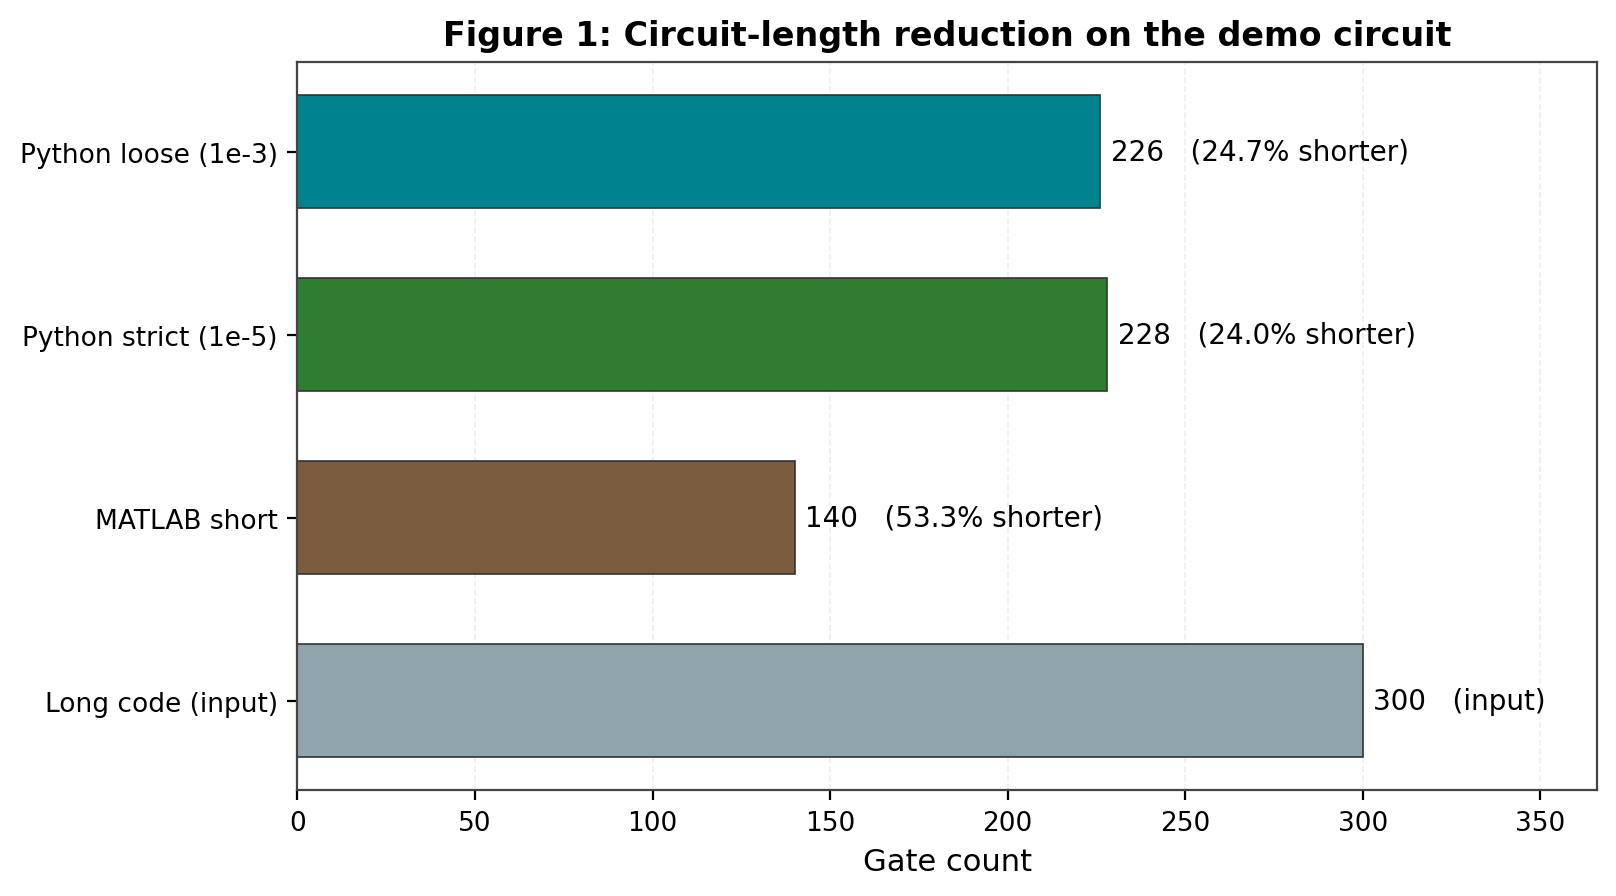
\includegraphics[width=0.85\linewidth]{../figures/figure1_motivation.png}
    \caption{Figure 1: circuit-length comparison between original and reduced variants.}
    \label{fig:motivation}
\end{figure}

\begin{figure}[H]
    \centering
    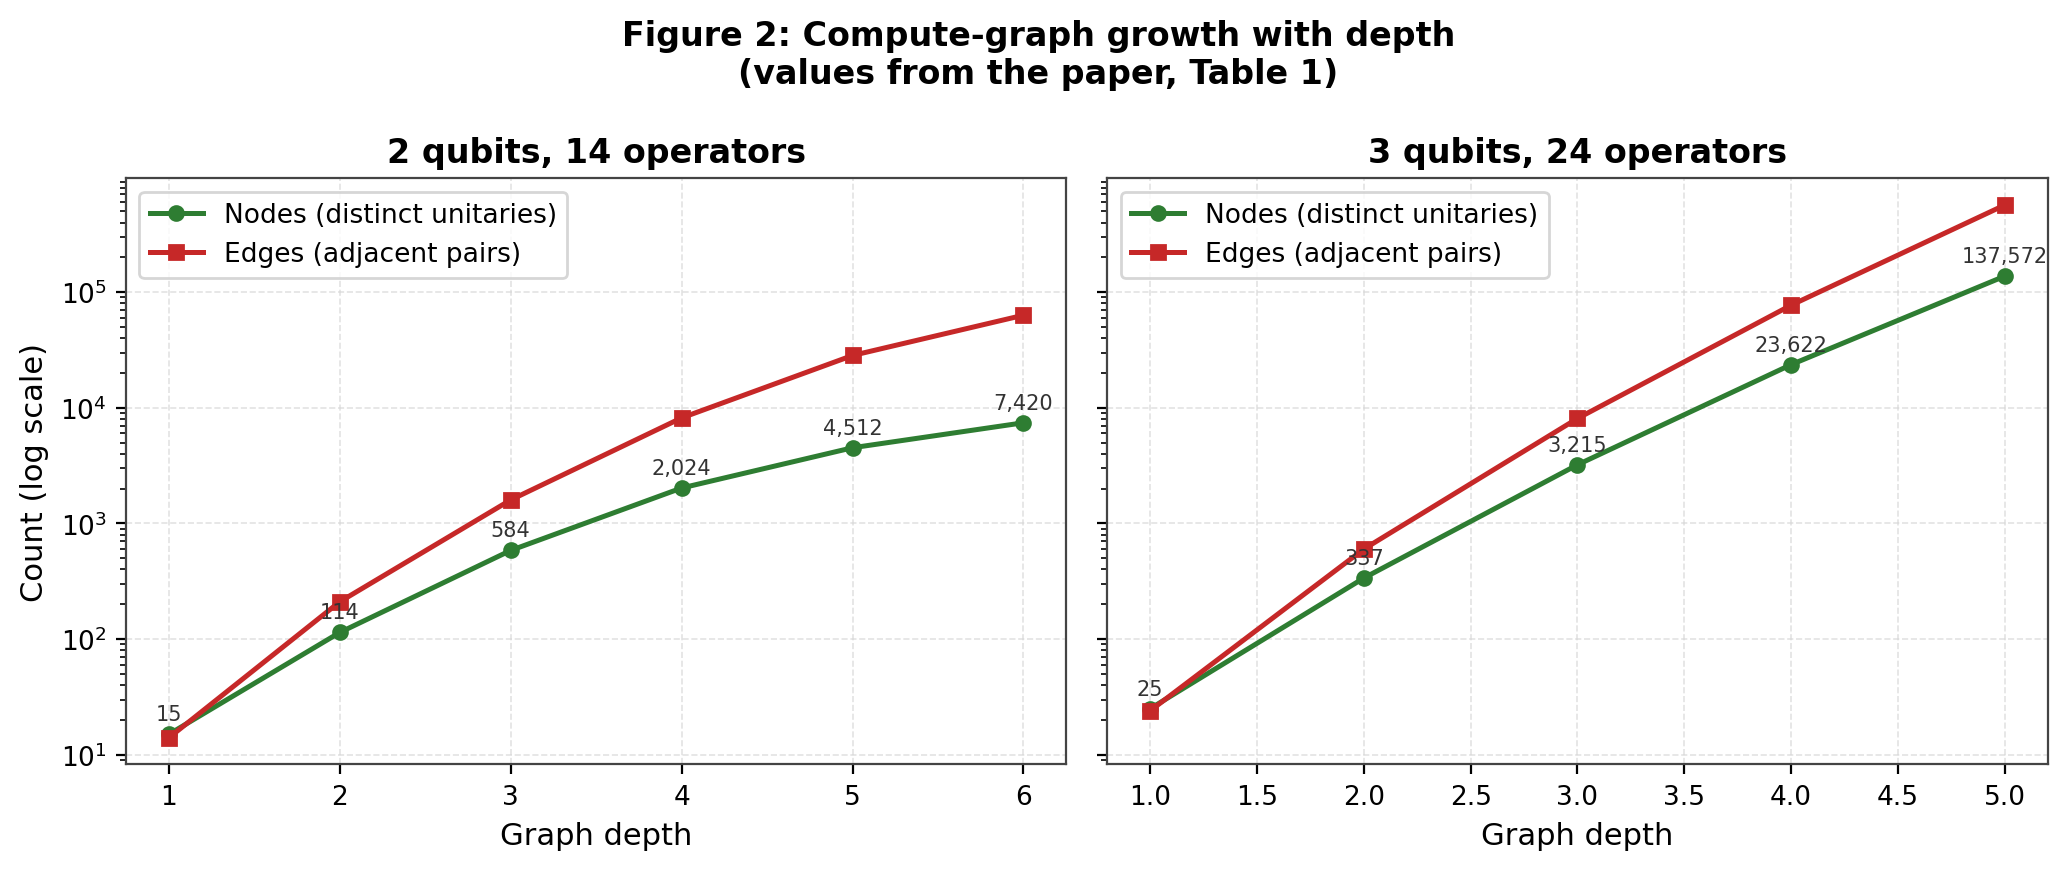
\includegraphics[width=0.95\linewidth]{../figures/figure2_compute_graph_growth.png}
    \caption{Figure 2: compute-graph growth with depth (values from the paper, Table 1).}
    \label{fig:graphgrowth}
\end{figure}

\begin{figure}[H]
    \centering
    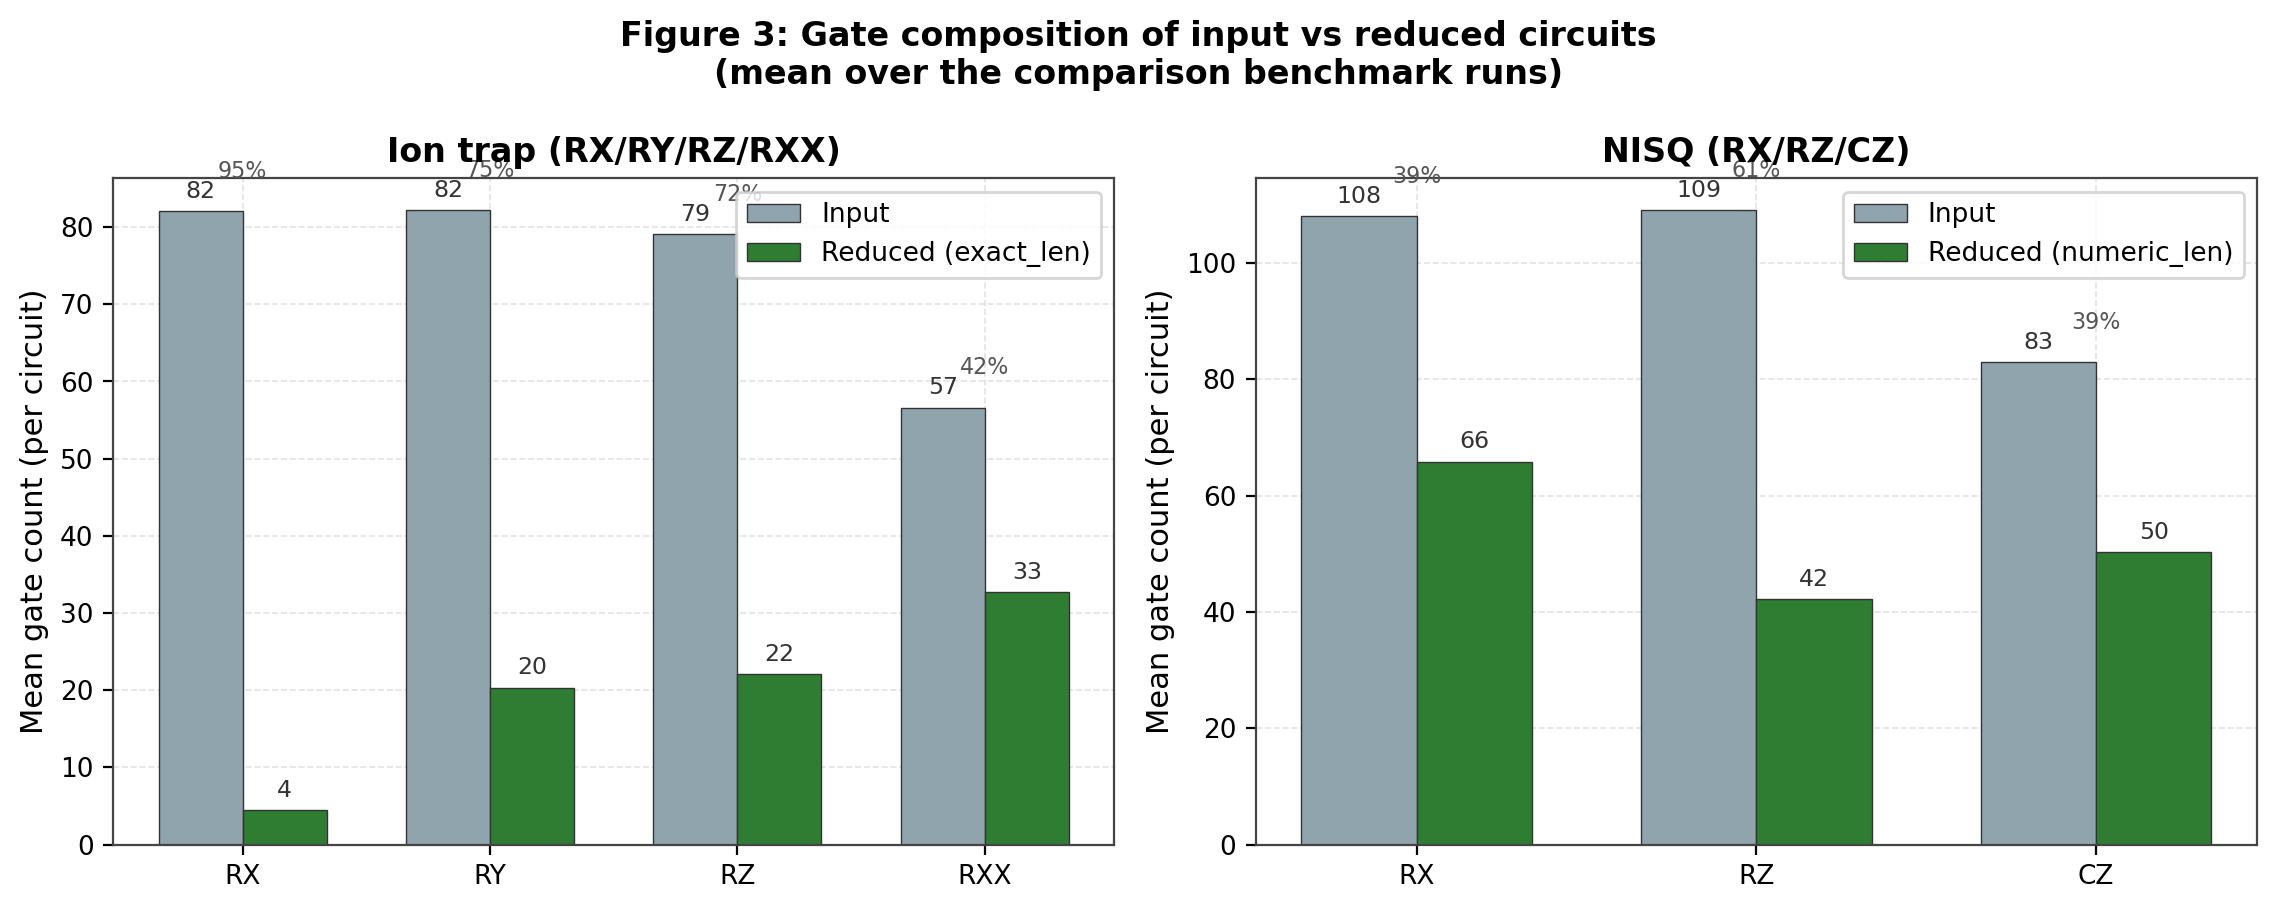
\includegraphics[width=0.95\linewidth]{../figures/figure3_pipeline.png}
    \caption{Figure 3: gate composition of input vs reduced circuits (mean over the comparison runs).}
    \label{fig:pipeline}
\end{figure}

\begin{figure}[H]
    \centering
    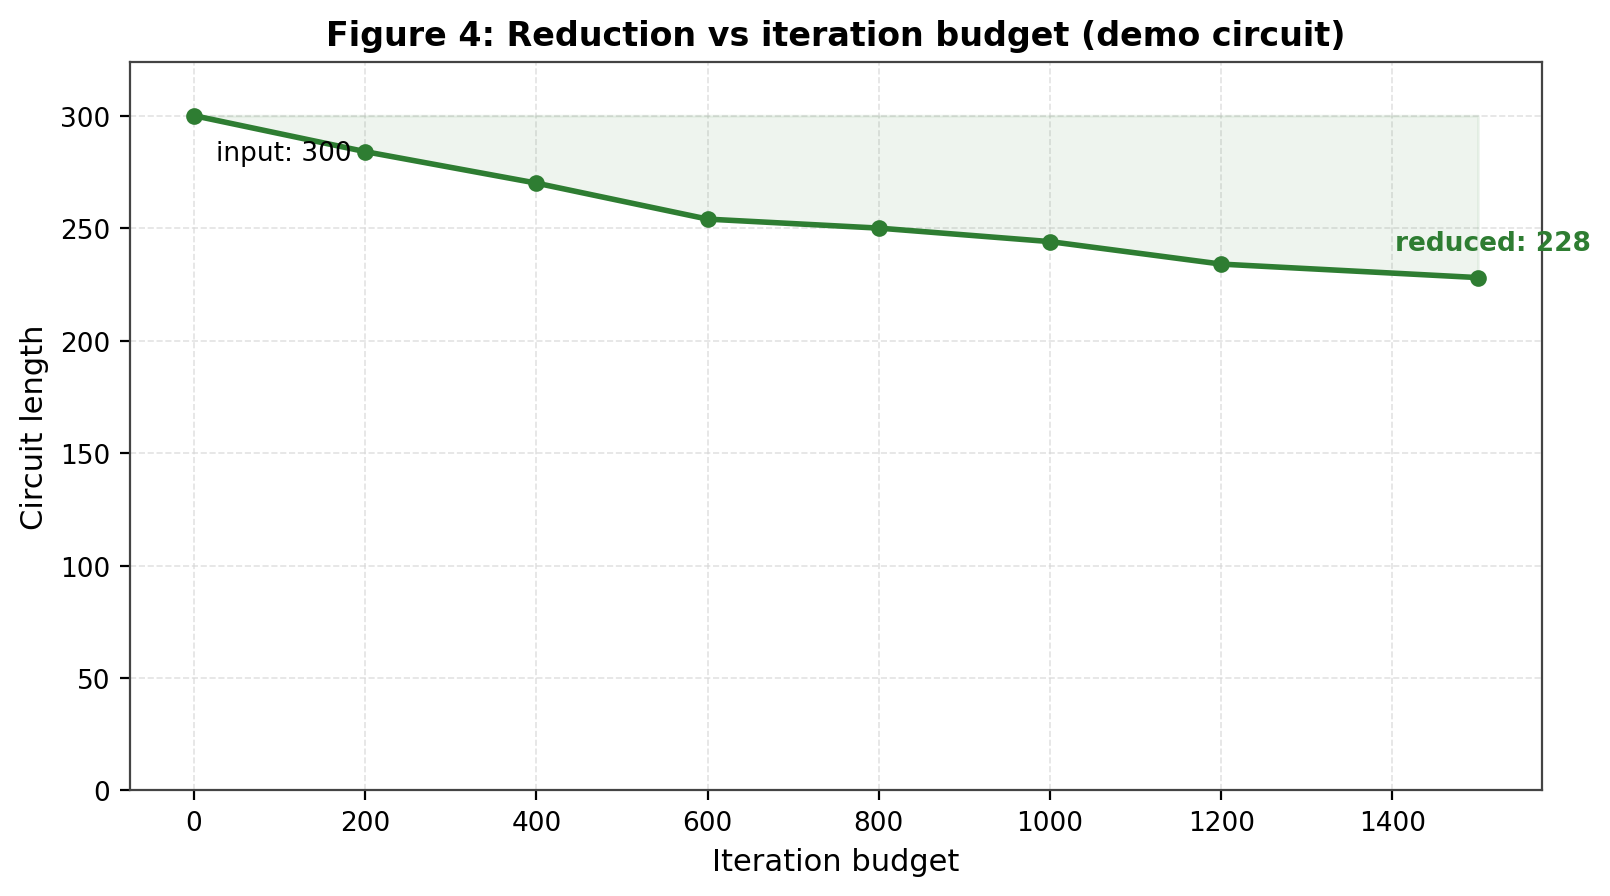
\includegraphics[width=0.85\linewidth]{../figures/figure4_reduction_curve.png}
    \caption{Figure 4: reduction trend versus iteration budget.}
    \label{fig:curve}
\end{figure}

\begin{figure}[H]
    \centering
    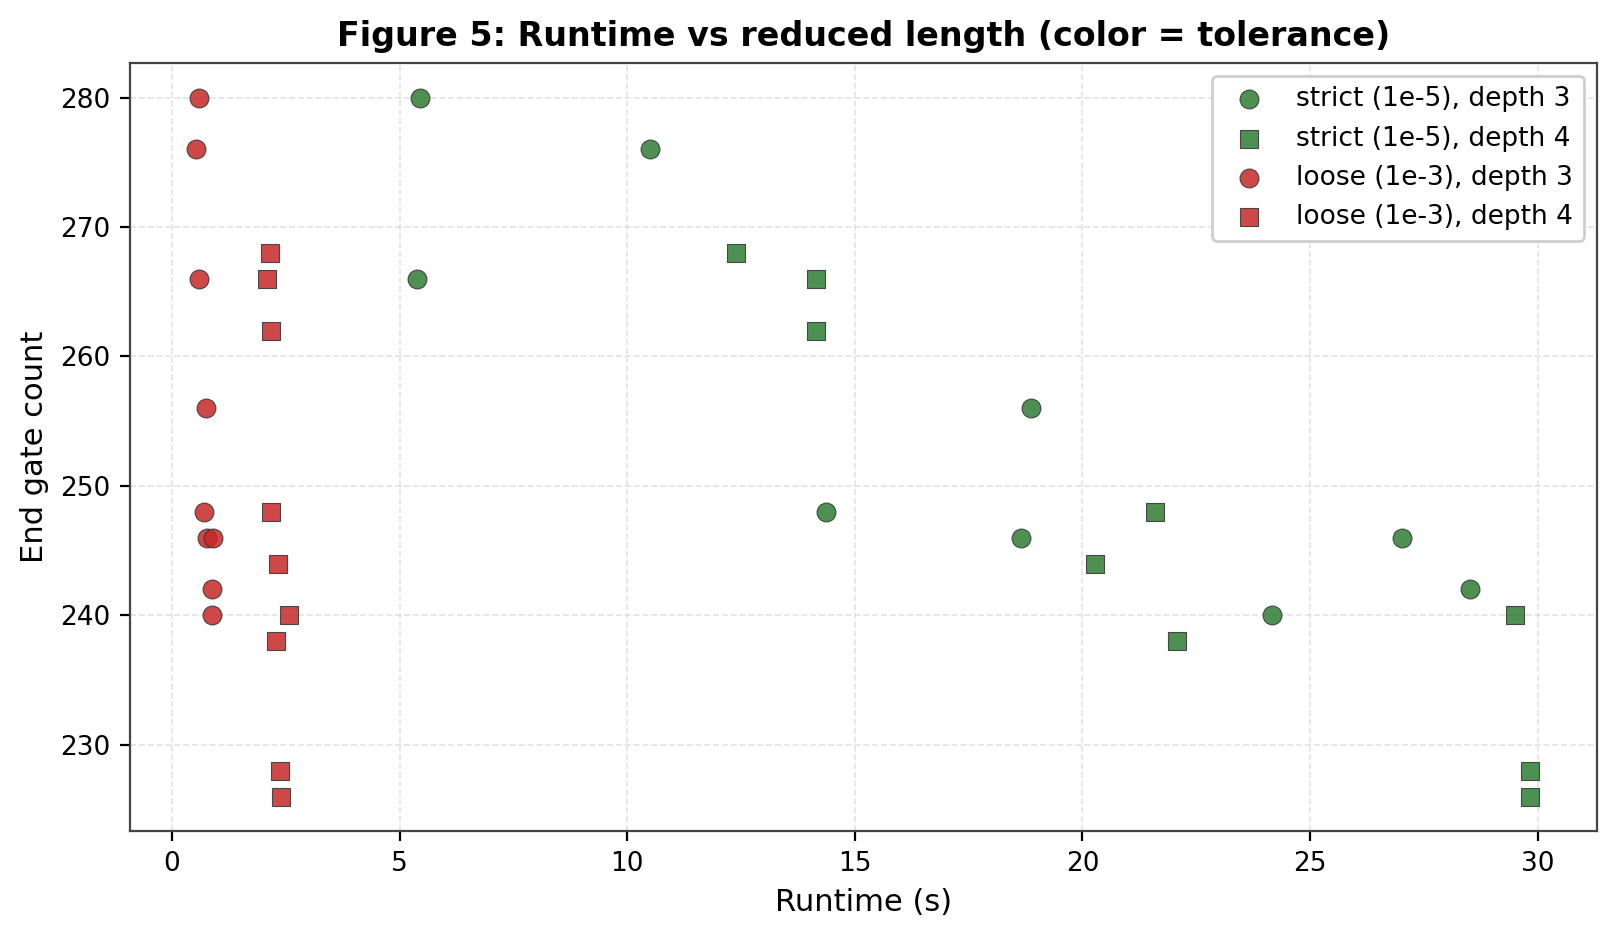
\includegraphics[width=0.85\linewidth]{../figures/figure5_runtime_vs_length.png}
    \caption{Figure 5: runtime versus achieved end length across benchmark runs.}
    \label{fig:runtime}
\end{figure}

\begin{figure}[H]
    \centering
    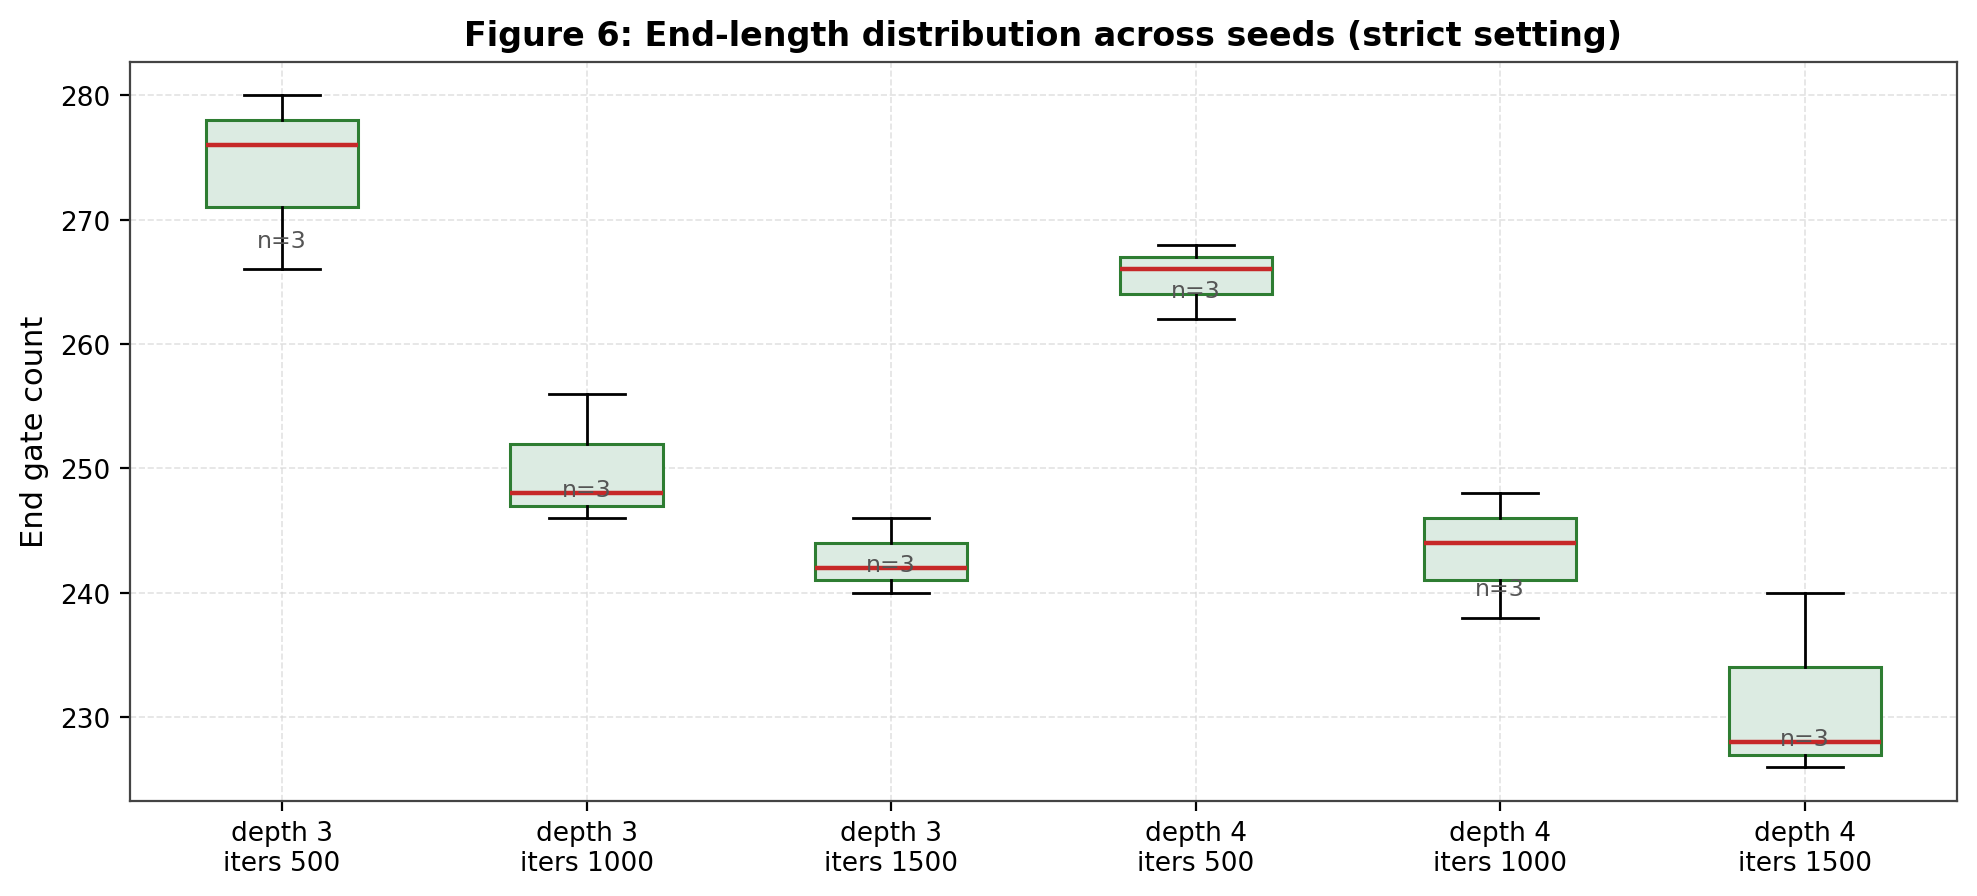
\includegraphics[width=0.95\linewidth]{../figures/figure6_boxplot.png}
    \caption{Figure 6: distribution of end lengths across seeds (strict setting).}
    \label{fig:boxplot}
\end{figure}

\begin{figure}[H]
    \centering
    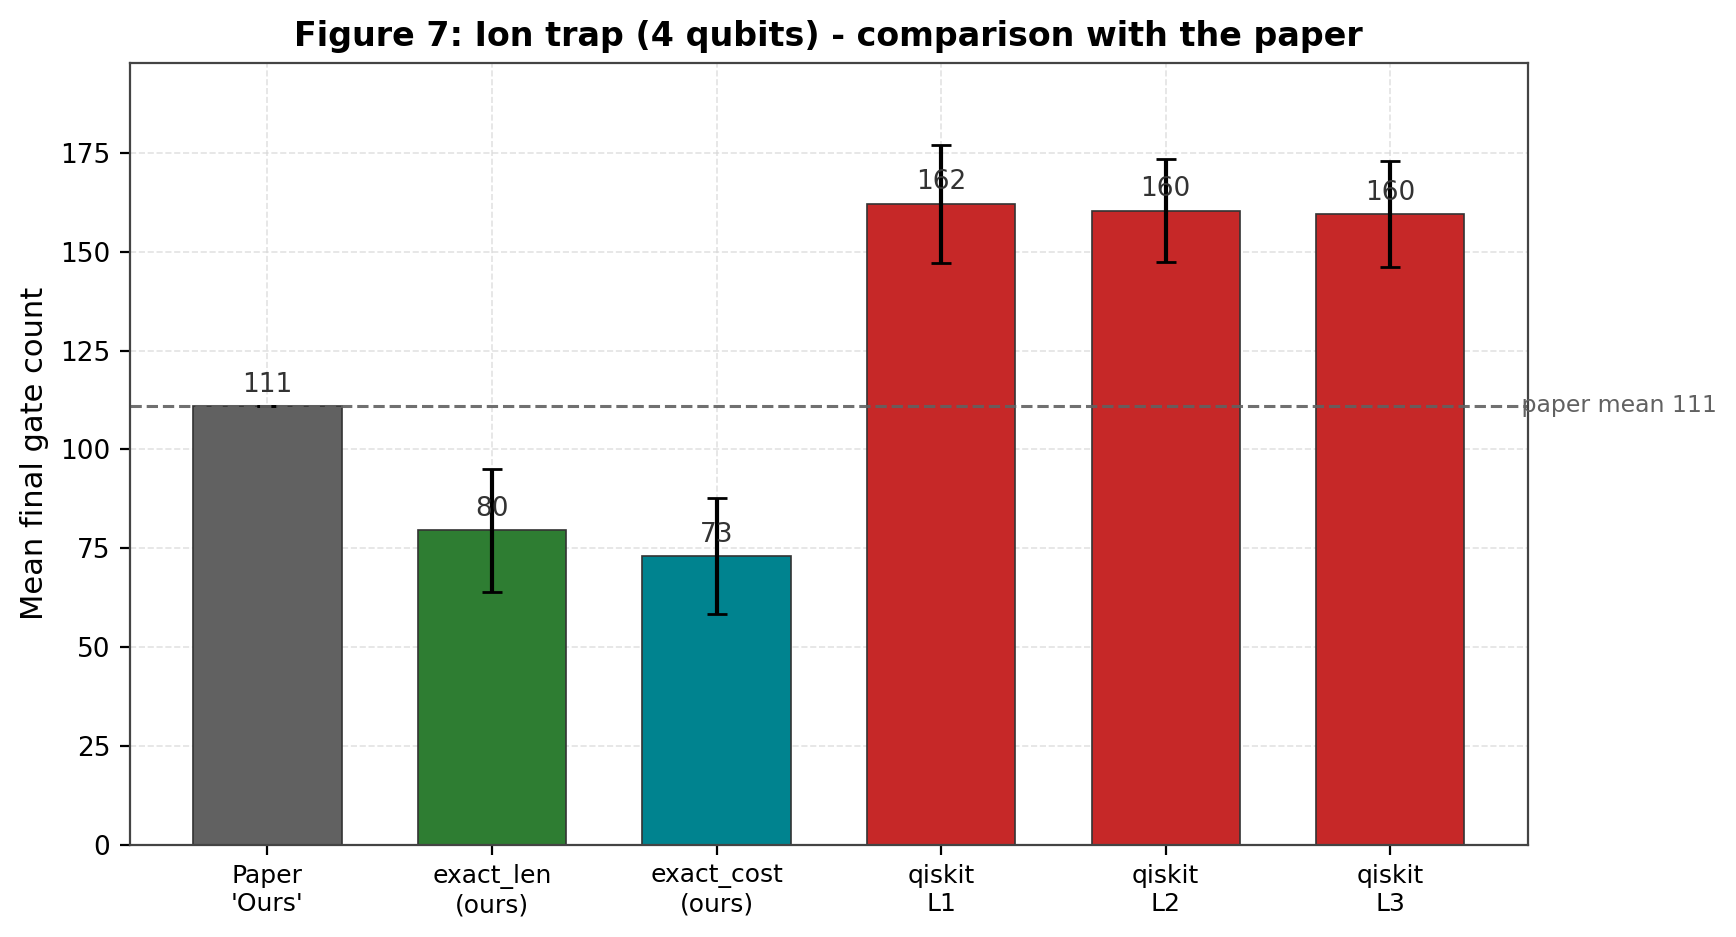
\includegraphics[width=0.9\linewidth]{../figures/figure7_comparison_ion_trap.png}
    \caption{Figure 7: ion-trap (4 qubits) -- comparison with the paper's 111-gate mean.}
    \label{fig:comp-ion}
\end{figure}

\begin{figure}[H]
    \centering
    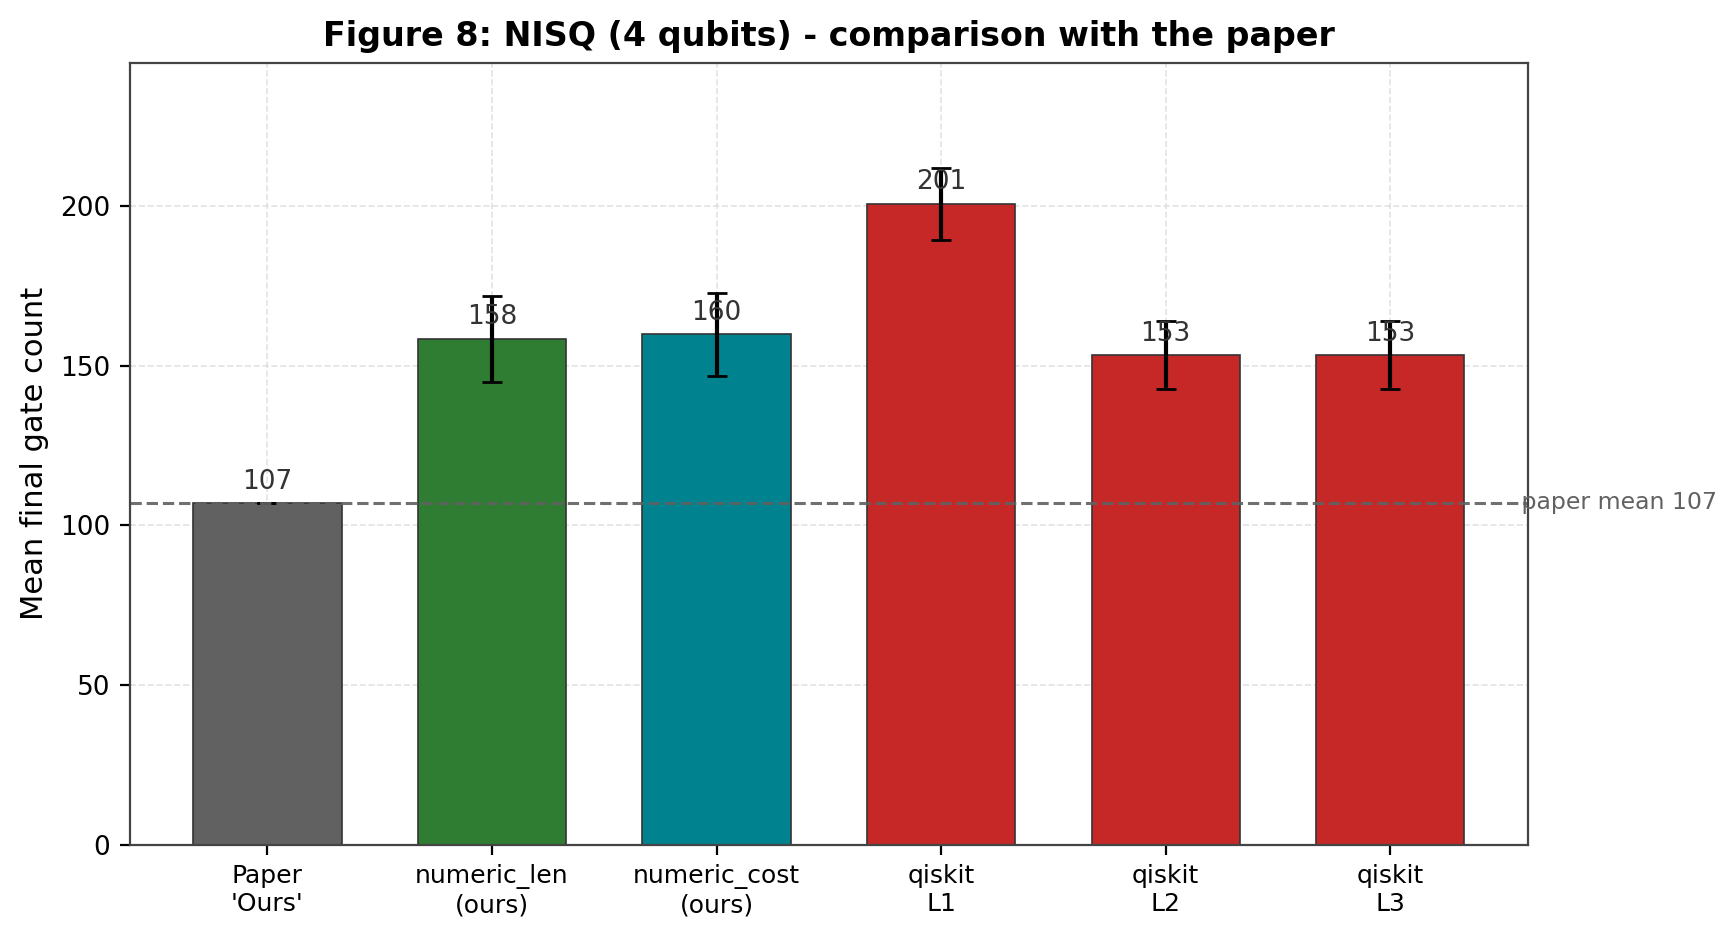
\includegraphics[width=0.9\linewidth]{../figures/figure8_comparison_nisq.png}
    \caption{Figure 8: NISQ (4 qubits) -- the gap to the paper's 107-gate mean.}
    \label{fig:comp-nisq}
\end{figure}

\begin{figure}[H]
    \centering
    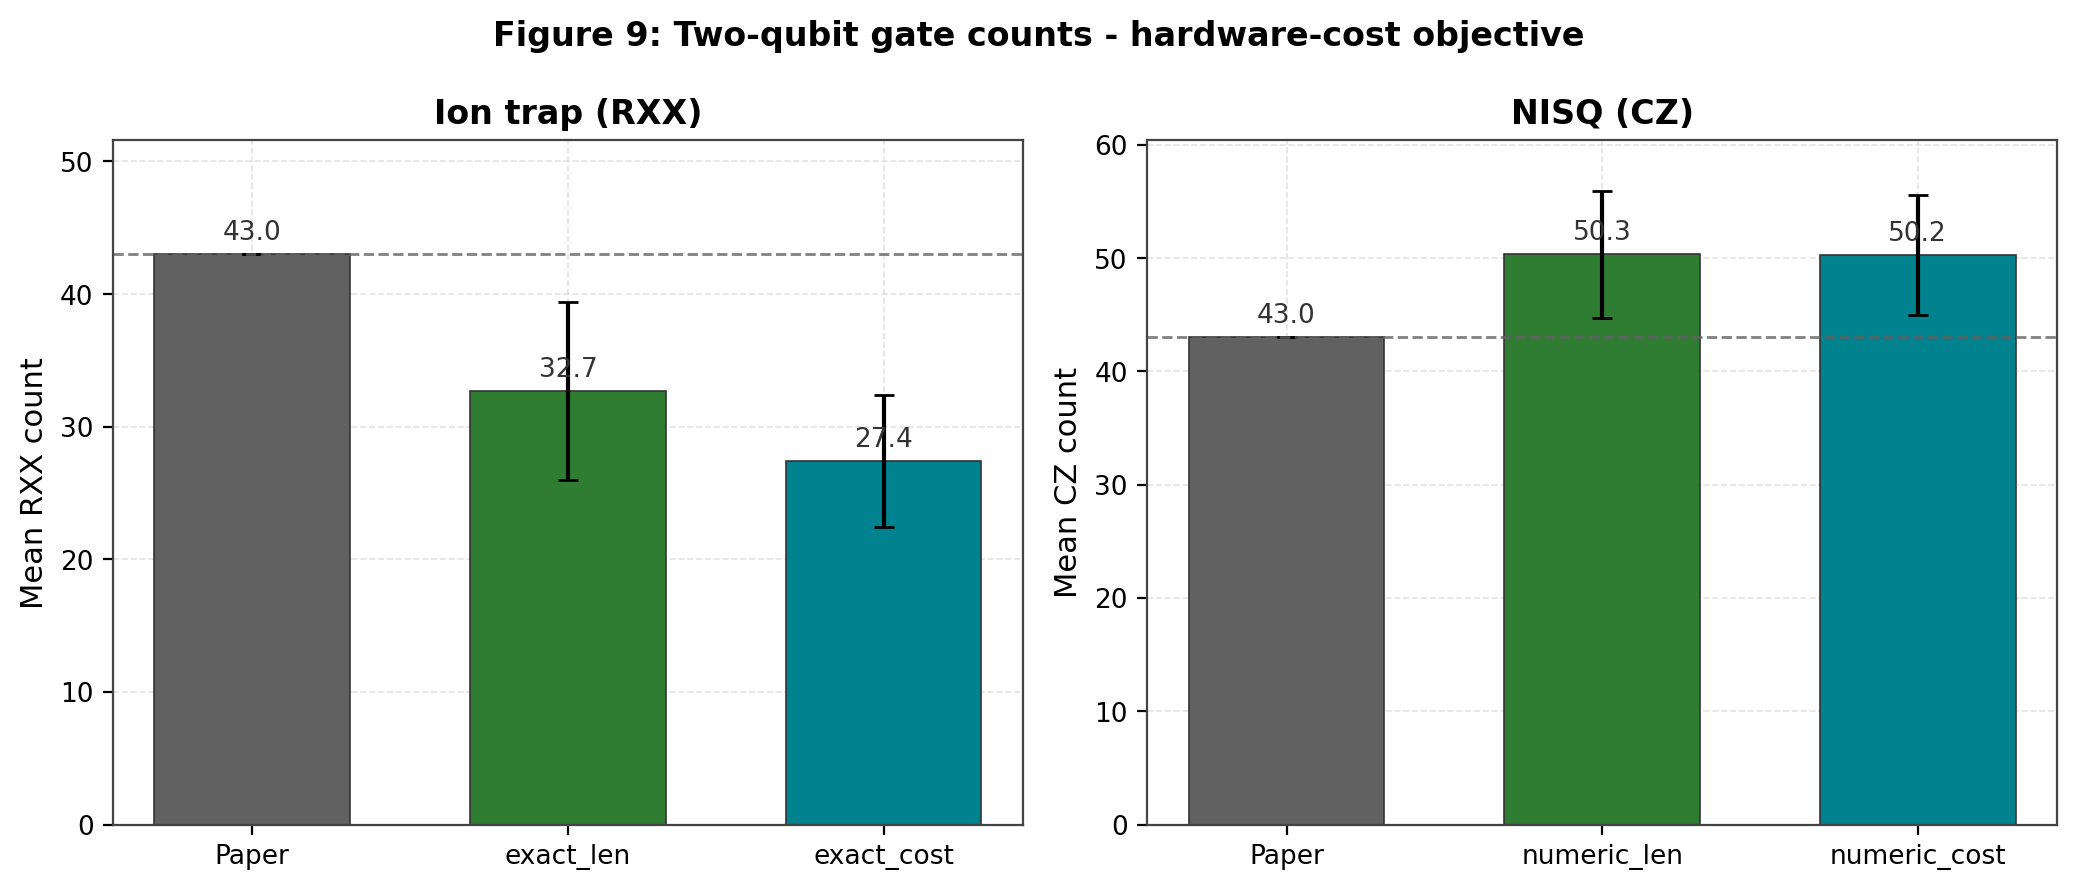
\includegraphics[width=0.95\linewidth]{../figures/figure9_two_qubit_counts.png}
    \caption{Figure 9: two-qubit gate counts (RXX/CZ) -- the hardware-cost objective.}
    \label{fig:comp-twq}
\end{figure}

\section{Discussion}
The paper's core behavior is reproduced: local stochastic search plus
compute-graph lookup reduces circuit length substantially. Three lessons stand
out. First, \emph{validation criteria drive conclusions}: strict (1e-5) checks
reject some reductions that loose (1e-3) checks accept, so both views must be
reported side by side. Second, \emph{exactness is achievable and stronger}: a
bit-exact symplectic lookup removes tolerance fragility entirely and reduces
further than the paper's reported results on the ion-trap gate set (73.0 vs.\
111 gates; 27.4 vs.\ 43 RXX), including the decoherence-relevant two-qubit
count the paper defers to future work. Third, \emph{baseline fidelity
matters}: reproducing the paper's qiskit baselines on NISQ (153.3 vs.\ 149)
validates the comparison framework, while the ion-trap baseline offset warns
that compiler versions shift absolute numbers.

\section{Future work}
\texttt{future\_work/} contains the baseline-parity and hardware probes
(\texttt{baseline\_parity\_results.csv}, \texttt{hardware\_metrics.json},
\texttt{future\_work\_status.md}):
\begin{itemize}
    \item Local method (strict): 228 gates in 2.4\,s, equivalence passed.
    \item qiskit transpile baseline on the same basis: opt0 300, opt1 229, opt2 219, opt3 219 gates.
    \item BQSKit 1.2.1 installed and import-verified; full pass-parity requires a dedicated pass mapping for this gate set.
    \item Hardware metrics: no authenticated provider available in this environment (explicitly logged as unavailable).
\end{itemize}
The main open lever is NISQ: the exact engine is Clifford-only, and the numeric
NISQ pipeline still trails the paper (159 vs.\ 107) for database-memory reasons
documented in \S\ref{sec:comparison}. Larger-memory machines and the
\texttt{--deep} graphs are the expected path to narrowing it.

\section*{Reproducibility note}
All outputs cited in this report are generated by scripts in \texttt{scripts/}
and committed under \texttt{results/}, \texttt{figures/}, \texttt{report/}, and
\texttt{future\_work/}. Figures regenerate with
\texttt{PYTHONPATH=src python scripts/generate\_figures.py}; the comparison
benchmark reruns with \texttt{scripts/benchmark\_comparison.py} (see README).

\end{document}
